%!TEX root = main.tex
\setcounter{chapter}{3}
\setcounter{section}{8}
\setcounter{theorem}{0}
\setcounter{equation}{0}

\lectureheader{161}{Calculus I}{Related rates}{\textit{Thomas' Calculus} \thesection}

\begin{remark}\,
\begin{itemize}
\item Given any equation that relates two of more variables, we can imagine that each of the variables is changing as functions of \textit{time} $t$.
\item We can then implicitly differentiate the equation with respect to $t$ to deduce a relationship between the \textit{rates} at which the different variables are changing with respect to time.
\item The class of problems for which this technique applies are called \textbf{related rates problems}.
\end{itemize}
\end{remark}

\begin{example}
A person's \textbf{cardiac output} is defined to be
\begin{equation*}
y = \frac{Q}{D},
\end{equation*}
where $Q$ is the volume of \si{CO_2} exhaled per time and $D$ is the difference between the \si{CO_2}-concentration in the blood pumped to the lungs and the \si{CO_2}-concentration in the blood returning from the lungs.
Suppose that $Q=233$ \si{mL/min}, $D=41$ \si{mL/L}, and $D$ is decreasing at a rate of 2 \si{mL/L/min} but $Q$ remains unchanged.
What is happening to the cardiac output?
\end{example}

\newpage

\begin{example}
Water runs into a conical tank at the rate of 9 \si{ft^3/min}.
The tank stands point down and has a height of 10 \si{ft} and a base radius of 5 \si{ft}.
How fast is the water level rising when the water is 6 \si{ft} deep?
\end{example}

\newpage

\begin{remark}\,
\begin{itemize}
\item Sometimes we are given a model (i.e., equation) for our problem; sometimes we have to construct one.
\item If you need to construct your own, do the following.
\begin{enumerate}
\item Draw picture.
\item Introduce notation (i.e., symbols/variables) to denote any quantities that are changing over time $t$.
\item Write down \underline{what you know} and \underline{what you want to know} in terms of this notation.
\item Decorate your picture with your notation.
\item Use your picture to write a model (i.e., equation(s)) that captures the relevant relationships between the relevant quantities (i.e, symbols/variables).
\item Implicitly differentiate with respect to $t$.
\item Evaluate and solve for the desired quantity.
\end{enumerate}
\end{itemize}
\end{remark}

\begin{example}
A hot air balloon rising straight up from a level field is tracked by a range finder 150 meters from the liftoff point.
At the moment that the range finder's elevation angle is $\pi/4$, the angle is increasing at a rate of 0.14 \si{min^{-1}}.
How fast is the balloon rising at that moment?
\end{example}

\newpage

\begin{example}
The figure below shows a rope running through a pulley at $P$ and bearing a weight $W$ at one end.
The other end is held 5 \si{ft} above the ground in the hand $M$ of a worker.
Suppose the pulley is 25 \si{ft} above the ground, the rope is 45 \si{ft} long, and the worker is walking away from the vertical line $PW$ at a rate of 4 \si{ft/sec}.
How fast is the weight being raised when the worker's hand is 21 \si{ft} away from $PW$?
\end{example}
\begin{flushright}
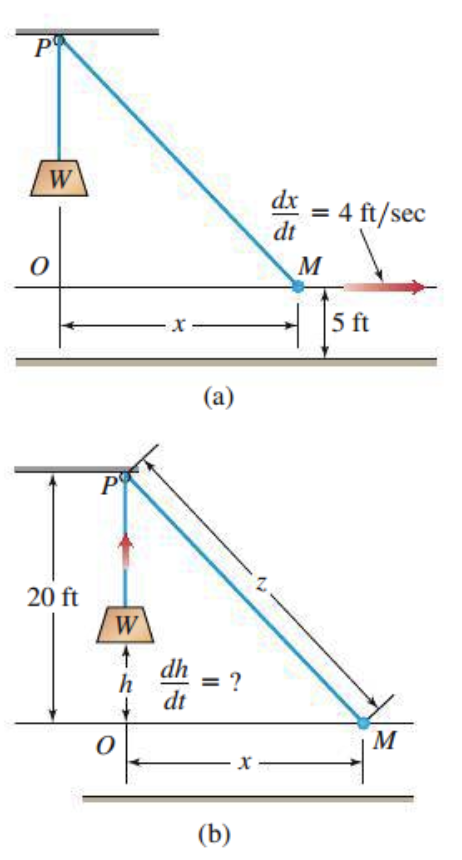
\includegraphics[width=1.5in]{img/pulley}
\end{flushright}

\newpage

\begin{example}
Coffee is draining from a conical filter into a cylindrical coffeepot at the rate of 10 \si{in^3/min}.
How fast is the level in the pot rising when the coffee in the cone is 5 \si{in} deep?
How fast is the level in cone the falling at that same moment?
\begin{flushright}
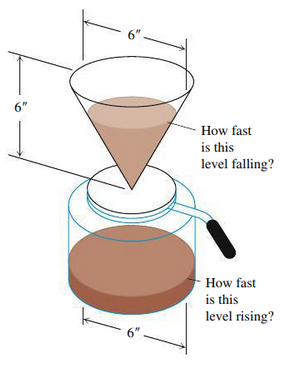
\includegraphics[width=2in]{img/coffee_maker}
\end{flushright}
\end{example}
